\documentclass{ci5652}
\usepackage{graphicx,amssymb,amsmath}
\usepackage[utf8]{inputenc}
% \usepackage[spanish]{babel}
\usepackage{hyperref}
\usepackage{subfigure}
\usepackage{paralist}
\usepackage[ruled,vlined,linesnumbered]{algorithm2e}
\usepackage{csvsimple}
\usepackage[none]{hyphenat}

\graphicspath{{graphics/}}
%-------------------------- Macros and Definitions ----------------------------%

% Add all additional macros here, do NOT include any additional files.

% The environments theorem (Theorem), invar (Invariant), lemma (Lemma),
% cor (Corollary), obs (Observation), conj (Conjecture), and prop
% (Proposition) are already defined in the ci5652.cls file.

%------------------------------------------------------------------------------%
%                                                                              %
%                                  TÍTULO                                      %
%                                                                              %
%------------------------------------------------------------------------------%

\title{Metaheurísticas para el problema de Aprendizaje de Pesos en Características}

\author{Stefani Castellanos
        \and
        Erick Silva}

%------------------------------------------------------------------------------%
%                                                                              %
%                                CONTENIDO                                     %
%                                                                              %
%------------------------------------------------------------------------------%

\begin{document}
\thispagestyle{empty}
\maketitle

%------------------------------------------------------------------------------%
%                                 RESUMEN                                      %
%------------------------------------------------------------------------------%

\begin{abstract}
*Inserte una descripción breve del paper.*

Palabras claves: Aprendizaje de Pesos en Características, Metaheurísticas,
\textit{Machine Learning}.
\end{abstract}

%------------------------------------------------------------------------------%
%                                INTRODUCCIÓN                                  %
%------------------------------------------------------------------------------%

\section*{Introducción}
% NO ESTÁ COMPLETO
Debido a la gran cantidad de información manejada actualmente, ha surgido la
necesidad de reducir el tamaño de dichos datos, sin embargo, esto genera el
problema de escoger correctamente que información es relevante para el
clasificador.\cite{Cano_2003} \\

Reducir el tamaño de los datos es posible a través de los siguientes métodos:

\begin{itemize}
  \item Seleccionando características del conjunto de datos, lo que reduce el
  tamaño de las columnas.
  \item Eliminando las instancias del conjunto de datos que aporte poca
  información.
  \item Determinando la importancia de las características, ya que proporciona
  información que permite guiar al clasificador y así, reducir el tiempo de
  procesamiento.
\end{itemize}

Este trabajo se enfocará en esta última, denominado el problema de Aprendizaje
de Pesos en Características. Se utilizará un algoritmo \textit{greedy} (ávido)
denomindado RELIEF, dos metaheurísticas de trayectoría y dos poblacionales,
para finalmente compararlas y determinar cual de ellos es más adecuado para el
problema.

%------------------------------------------------------------------------------%
%                          DESCRIPCIÓN DEL PROBLEMA                            %
%------------------------------------------------------------------------------%

\section{Descripción del problema}

Antes de describir el problema APC, es necesario comprender en qué consiste
un problema de clasificación; se dispone de un conjunto de posibles clases
($C$) y un conjunto de datos ($X$), en donde una instancia $x_i$ es un vector
previamente clasificado y de la forma:
$$x_i = \langle f_1, f_2, \dots, f_n, c\rangle $$ en donde:

\begin{itemize}
  \item $f_i$ : el valor de cada característica.
  \item $n$ : la cantidad de característcas.
  \item $c$ : la clase a la que pertenece dicha instancia, con $c \in C$.
  \item $|X| = m$: cantidad de instancias.
  \item $|C| = p$ : cantidad de clases.
\end{itemize}

Es común particionar $X$ en dos subconjuntos que representen el conjunto de
entrenamiento y el de prueba, $X_e$ y $X_p$ respectivamente. $X_e$ es utilizado
para que el algoritmo aprenda los parámetros que le permitan clasificar
correctamente todas sus instancias y así, utilizar $X_p$ para validar los
resultados obtenidos.\\

El problema del Aprendizaje de Pesos en Características consiste en optimizar el
rendimiento de un clasificador, a partir de la inclusión de pesos asociados a
las características del conjunto de datos. Los pesos ponderan la relevancia de
cada característica y modifican su valor al momento de calcular las distancias
entre instancias, de tal forma que los clasificadores que se construyan a partir
de estos, sean más certeros y/o más rápidos. En este caso en particular, el
clasificador considerado será el \textit{K-Nearest Neighbor} (K-vecinos más
cercanos) con $K=1$ (1-NN).\\

El algoritmo K-NN asume que todas las instancias corresponden a puntos en un
espacio $n$-dimensional ($\Re^n$), en donde $n$ es la cantidad de
características del conjunto de datos. \cite{Mitchell_1997}. El algoritmo es el
siguiente:

\begin{algorithm}
 \DontPrintSemicolon
 \vspace*{0.1cm}
 \KwIn{Conjunto de entrenamiento $X_e$, Conjunto de prueba $X_p$, $K$}
 \KwOut{Conjunto $X_p$ clasificados según $C$}
  \ForEach{$x_i \in X_p$}{
   vecinos = [ ];\;
   \ForEach{$x_j \in X_e$}{
    d = distancia($x_i, x_j$);\;
    agregar($x_j, d, vecinos$);\;
   }
  k\_vecinos = seleccionar\_cercanos($k, vecinos$);\;
  clasificar($x_i, k\_vecinos$);\;
 }
 \KwRet{$X_p$ clasificado}
 \vspace*{0.1cm}
 \caption{K-Nearest Neighbor}
\end{algorithm}

El proceso de aprendizaje de este clasificador consiste en almacenar una tabla
con las instancias correspondientes al $X_e$ junto a la clase asociada a cada
uno de ellos. Dado una instancia $x_i \in X_p$, se calcula su distancia a todas
las otras que pertenecen al conjunto de entrenamiento y se escogen las $k$ más
cercanas \cite{Herrera_2017}; usualmente se determina la proximidad entre dos
ejemplos utilizando la distancia Euclideana. Finalmente, $x_i$ se clasifica
según la clase mayoritaria grupo y se retorna el conjunto de pruebas clasificado.
%ORDEN DE K-NN

%-------------------------- FUNCIÓN OBJETIVO ----------------------------------%

\subsection{Función objetivo}

Al ser APC un problema de optimización, es necesario establecer cuál es la
función que se desea mejorar. En este caso, dadas las características del
problema, resulta evidente que obtener una "buena" solución está fuertemente
relacionado con la cantidad de instancias clasificadas correctamiente usando
1-NN. El objetivo es encontrar el mejor vector de pesos que permita máximizar la
tasa de aciertos del clasificador 1-NN. Más específicamente:

\begin{equation}
  \max\ tasa(\text{1-NN}(X, W)) = 100 \times \frac{aciertos(X)}{total(X)}
\end{equation}

sujeto a:
\[
w_i = [0, 1] \ \ 1 \leq i \leq n
\]

donde:
\begin{itemize}
  \item $W = \langle w_1, \dots, w_n\rangle$ es una solución al problema.
  \item 1-NN es el clasificador k-NN con $k=1$ vecinos, generado a partir del
  conjunto de datos inicial.
  \item $X$ es el conjunto de datos sobre el cual se evalúa el clasificador.
  \item $aciertos$ es la cantidad de instancias de $X$ clasificadas
  correctamente por 1-NN.
  \item $total$ es la cantidad total de instancias de $X$.
\end{itemize}

%---------------------- REPRESENTACIÓN DE LA SOLUCIÓN -------------------------%

\subsection{Representación de la solución}

La solución al problema de Aprendizaje de Pesos en Características viene dado
por $W = \langle w_1, \dots, w_n\rangle$, un vector de números reales de tamaño
$n$ (cantidad de características) en el que el valor de cada $w_i$  define el
peso que pondera a la  característica $f_i$, es decir, representa que tan
importante es para distinguir a que clase pertenece un ejemplo.\\

Cada $w_i$ debe pertenecer al intervalo $[0,1]$; los valores cercanos a 1 indican
que la característica es más importante. En caso de que algún valor quede fuera
de este intervalo, se debe normalizar, seleccionando el máximo valor del vector
y dividiendo todos los valores entre dicho número.

%------------------------------------------------------------------------------%
%                             ALGORITMO RELIEF                                 %
%------------------------------------------------------------------------------%
\section{Algoritmo Relief}

Las metaheurísticas suelen ser inicializadas con soluciones generadas
aleatoriamente, sin embargo, esto puede producir un retardo en la ejecución o
desembocar en una convergencia prematura en un óptimo local, por lo que se
requiere de un algoritmo eficiente que tome información del problema y guie las
búsqueda de manera inteligente. Para el problema considerado en este artículo,
existe tal heurística: Relief.\\

Relief, es un algoritmo de selección de características inspirado en el
aprendizaje basado en instancias, detecta aquellos ejemplos que son
estadísticamente relevantes para el concepto objetivo en tiempo lineal
($\Theta(nmp)$). Utiliza un \textit{threshold}, $\tau$ entre
$0 \leq \tau \leq 1$ , que codifica la relevancia de una característica en
particular \cite{Kira_1992};  en esta versión será omitido este parámetro puesto
que las metaheurísticas utilizan el vector de pesos y no el vector de
relevancias que se obtiene con $\tau$.\\

Relief utiliza la distancia euclideana $n$-dimensional para determinar el "amigo
más cercano" y el "enemigo más cercano" de una instancia $x_i$. Se denomina a
una instancia "amigo más cercano" o "near-hit" a la instancia que pertenezca a
la misma clase de $x_i$ y se encuentre a menor distancia. Se denomina a una
instancia "enemigo más cercano" o "near-miss" a la instancia que pertenezca a
una clase diferente a $x_i$ y se encuentre a menor distancia \cite{Kira_1992}.

\begin{algorithm}
 \DontPrintSemicolon
 \vspace*{0.1cm}
 \KwIn{Conjunto de entrenamiento $X_e$}
 \KwOut{Vector de pesos $W$}
  W = {0, 0 \dots, 0}\;
  \ForEach{$x_i \in X_e$}{
   a = amigo\_mas\_cercano($x_i$);\;
   e = enemigo\_mas\_cercano($x_i$);\;
   \;
   /* Actualizar pesos de $W$ */\;
   \For{$i \dots n$}{
    dif\_amigo = diferencia($x_i, a$);\;
    dif\_enemigo = diferencia($x_i, e$);\;
    $w_i$ = $w_i$ - dif\_amigo + dif\_enemigo;\;
   }
  }
  normalizar($W$);\;
 \KwRet{$W$}
 \vspace*{0.1cm}
 \caption{Relief}
\end{algorithm}

La diferencia entre el valor $x_i$ y el amigo/enemigo más cercano está definido
por: \\
- Para los atributos con valores numéricos:
$$\text{diferencia}(a,b) = {(a - b)}^{2}$$
- Para los atributos con valores nominales:
\[
\text{diferencia}(a,b) =
  \begin{cases}
    0 & \text{son el iguales}\\
    1 & \text{son diferentes}
  \end{cases}
\]
%------------------------------------------------------------------------------%
%                              METAHEURÍSTICAS                                 %
%------------------------------------------------------------------------------%

\section{Metaheurísticas}

Las soluciones a muchos problemas de optimización son intratables, es decir,
obtener la mejor respuesta podría tomar un tiempo potencialmente infinito, no
ser resoluble o no se dispone de la capacidad computacional suficiente para
resolverlo. Las metaheurísticas constituyen un conjunto de estrategías para
guiar heurísticas en la tarea de encontrar soluciones aceptables en un tiempo
razonable para resolver un problema difícil o del que no se dispone información
completa \cite{Talbi_2009}. Usualmente poseen un componente estocástico, por lo
que la solución depende de las variables aleatorias generadas y se describen los
resultados basados en observaciones empíricas. Existen tres tipos de
metaheurísticas: de trayectoria, poblacionales e hibridas.\\

En general, las meteheurísticas mejoran soluciones obtenidas anteriormente. Sus
componentes principales son:

\begin{itemize}
  \item Inicialización. Se requiere alguna solución inicial según la
  representación del problema particular, esta puede ser generada de manera
  aleatoria o utilizando algún algoritmo \textit{greedy}.
  \item Operador de vecindad. Se debe disponer de un algortimo que, a partir de
  otra solución, genere un conjunto de soluciones "vecinas". Este operador puede
  entenderse como una pequeña perturbación en alguna componente de la
  representación utilizada.
  \item Criterio de selección. Entre las soluciones que pertenecen a la
  vecindad, se debe escoger la "mejor". Existen diversas políticas, las más
  conocidas son: el mejor de toda la vecindad, el primer mejor y el mejor de una
  porción de la vecindad. Escoger algún criterio sobre otro depende del
  problema.
  \item Criterio de convergencia. Al mejorar una solución a partir de la
  anterior, es indispensable contar con algún mecanismo que permita detener la
  ejecución de la metaheurística y devolver alguna solución. Los más conocidos
  son: detenerse al encontrar el óptimo (si este es conocido), luego de un
  número fijo de iteraciones y luego de un número fijo de iteraciones sin
  modificar la mejor solución.

\end{itemize}

%--------------------- Metaheurísticas de trayectoria -------------------------%

\subsection{Metaheurísticas de trayectoria}

Al resolver un problema de optimización, las metaheurísticas de trayectoria,
utilizan una solución y realizan mejoras sobre esta, iterativamente; pueden ser
entendidas como "caminatas" sobre el espacio de búsqueda del problema.
Probablemente la metaheurística de trayectoria más conocida es
Local Search, que toma una solución inicial, encuentra sus vecinos y
escoge el mejor según un criterio \cite{Talbi_2009}.

\begin{algorithm}
 \DontPrintSemicolon
 \vspace*{0.1cm}
 \KwOut{Mejor solución s*}
  s* = gen\_sol();\;
  \While{!criterio\_convergencia()}{
    V = gen\_vecinos(s');\;
    s' = seleccionar\_mejor(V);\;
    \If{costo(s) $<$ costo(s)}{
      s = s';\;
    }
  }
 \KwRet{s}
 \vspace*{0.1cm}
 \caption{Local Search}
\end{algorithm}

%--------------------------- Iterated Local Search ----------------------------%

\subsubsection{Búsqueda Local Iterada (Iterated Local Search)}

Local Search podría quedar atrapado en un óptimo local y jamás llegar al global
ya que se función es intensificar la búsqueda en una vencindad. Para mitigar
este riegos se crea una de las metaheurísticas más fáciles de implementar:
Iterated Local search, que supone una mejora sobre LS. Primero se aplica LS a la
solución inicial; luego, en cada iteración, se realiza una perturbación del
óptimo local y se repite el proceso hasta un cumplir el criterio de aceptación
\cite{Talbi_2009}.\\

\begin{algorithm}
 \DontPrintSemicolon
 \vspace*{0.1cm}
 \KwOut{Mejor solución s*}
  s = gen\_sol();\;
  s* = local\_search(s);\;
  \While{!criterio\_convergencia()}{
    s = perturbar(s*);\;
    s' = local\_search(s');\;
    \If{$s* < s'$}{
      s* = s';\;
    }
  }
 \KwRet{s*}
 \vspace*{0.1cm}
 \caption{Iterated Local Search}
\end{algorithm}


%--------------------------- Simulated Annealing ------------------------------%

\subsubsection{Recocido Simulado (Simulated Annealing)}

Su nombre proviene del proceso físico de recocer sólidos, en el que un sólido
cristalino es calentado y luego se deja enfriar muy lentamente hasta que alcance
su configuración más estable y estructuralmente superior, por lo tanto está
libre de defectos del cristal \cite{Glover_2003}. En términos de resolver un
problema de optimización, el sólido representa una solución, "calentarlo" es
perturbar la solución hasta que la temperatura se estabilice y el "enfriamiento"
es una función no-creciente.\\

En cada iteración, Simulated Annealing, genera dos posibles soluciones: la
actual y otra, las cuales son comparadas. Aquellas que mejoren la actual
son siempre aceptadas; también existe una función probabilística dependiente de
la temperatura que permite aceptar alguna solución considerada "inferior" y así,
escapar de un mínimo local. Típicamente es una función no-creciente en cada
iteración del algoritmo y al aproximarse la temperatura a cero la probabilidad
de aceptar una solución que no mejora es menor \cite{Glover_2003}. La
temperatura sólo decrece cuando se ha alcanzado una condición de equilibrio.\\

\begin{algorithm}
 \DontPrintSemicolon
 \vspace*{0.1cm}
 \KwIn{$T\_inicial$}
 \KwOut{Mejor solución s}
  s = gen\_sol();\;
  T = T\_inicial;\;
  \While{!criterio\_convergencia()}{
    \While{!equilibrio}{
      /* Temperatura inicial */;\;
      s' = gen\_sol();\;
      \If{costo($s$) $<$ costo($s'$)}{
        s = s';\;
      }
      \Else{
        r = rand();\;
        delta = costo($s$) - costo($s'$);\;
        acep = 1/$\exp^{1 + exp( 1 + delta / T)};$\;
        \If{r $<$ acep}{
          s = s';\;
        }
      }
    }
    T = actualizar\_temp();\;
  }
 \KwRet{s}
 \vspace*{0.1cm}
 \caption{Simulated Annealing}
\end{algorithm}

%---------------------- Metaheurísticas poblacionales -------------------------%

\subsection{Metaheurísticas poblacionales}

La mayoría de estos algoritmos están inspirados en fenómenos naturales y el
comportamiento de los animales. Estas metaheurísticas toman una población
inicial que está constituida por un conjunto de posibles soluciones del
problema. Luego, iterativamente, se generan nuevos individuos (soluciones) a
través de "cruces" y mutaciones en los genes (componentes del vector), los
cuales son seleccionados para reemplazar a algunos de la actual población,
creando una nueva. Este proceso se repite hasta alcanzar un criterio de
convergencia dado \cite{Talbi_2009}.\\

Los cruces puede ser entendidos como una combinación de dos individuos de la
población para crea otros nuevos, preservando algunas características de los
originales. El operador de mutación efectúa una perturbación de un hijo
generado; el propósito de este es realizar variaciones en la población que
permitan explorar nuevos lugares en el espacio de solución, es decir,
diversificar la búsqueda.

%------------------------------- Scatter Search -------------------------------%

\subsubsection{Scatter Search}

Es un metaheurística evolutiva y poblacional que recombina soluciones
seleccionadas de un "conjunto de referencia" para construir otras nuevas. El
método comienza generando una población inicial cuyos individuos satisfacen un
criterio de diversidad y calidad. El conjunto de referencia es construido
seleccionando buenas representaciones de la población que se cruzan para proveer
otras iniciales y luego mejorarlas con procedimientos basados en metaheurísticas
de trayectoria como Local Search. De acuerdo con esto, el conjunto de referencia
es actualizado para que contenga soluciones de buena calidad y otras que
permitan diversificar la búsqueda. El proceso itera hasta que un criterio de
parada se satisface \cite{Talbi_2009}.\\

Scatter Search aprovecha la información proveída por una heurística para crear
las soluciones "buenas" e intensificar la búsqueda alrededor de estos espacios.

\begin{algorithm}
 \DontPrintSemicolon
 \vspace*{0.1cm}
 \KwIn{Población $P$}
 \KwOut{Mejor solución p\_mejor}
  $P$ = mejorar\_pop($P$);\;
  refSet = inicializar\_pop($P$);\;
  \While{!criterio\_convergencia()}{
    \ForEach{$r \in refSet$}{
      r = combinar(r, r');\;
    }
    refSet = mejorar\_ref(refSet);\;
    $P$ = actualizar($P$);\;
    p\_mejor = mejor($P$);\;
  }
 \KwRet{$p\_mejor$}
 \vspace*{0.1cm}
 \caption{Scatter Search}
\end{algorithm}

%--------------------------- Diferential Evolution ----------------------------%

\subsubsection{Differential Evolution}

Es un algoritmo evolutivo que genera su población inicial de manera aleatoria y
con un tamaño mayor o igual a 4. Suele utilizarse para problemas de optimización
contínuos pues cada individuo tiene componentes con números reales.\\

El operador de cruce que utiliza está basado en la combinación líneal de las
soluciones utilizando la distancia entre las mismas. Dado un padre $x$ y tres
otro individuos seleccionados aleatoriamente $r1, r2$ y $r3$, se crea un nuevo
vector $u = r1 + F(r2 - r3)$. $F$ representa un factor permite añadir un peso o
importancia a la diferencia entre $r2$ y es tal que $r3$ y $F \in (0, 1)$
\cite{Glover_2003}. Finalmente se reemplaza $p$, con $p'$, de la
siguiente manera:

\[
p'_i =
  \begin{cases}
    u_i & \text{si } rand < CR\\
    p_i & \text{si } rand \geq CR
  \end{cases}
\]

donde:
\begin{itemize}
  \item $CR \in (0,1)$ : \textit{Crossover Constant}, un parámetro que
  representa la probabilidad de cruce.
  \item $rand$ : el número aleatorio entre 0 y 1 para escoger un componente u
  otro.
  \item $1 \leq i \leq n $ : índice para cada característica.
\end{itemize}

\begin{algorithm}
 \DontPrintSemicolon
 \vspace*{0.1cm}
 \KwIn{Población $P$, $F, CR$}
 \KwOut{Mejor solución p\_mejor}
  \While{!criterio\_convergencia()}{
    \ForEach{$p \in P$}{
      \For{$i = 0 \dots n - 1$}{
        /* Mutar y cruzar */\;
        r = rand($0, 1$)\;
        \If{$r < CR$}{
          $u_i = r1_i + F(r2_i - r3_i)$;\;
        }
        \Else{
          $u_i = p_i$\;
        }
        /* Reemplazar según la regla */\;
        $p'_i$ = reemplazar($p_i, u_i$)
      }
    }
    p\_mejor = mejor($P$);\;
  }
 \KwRet{$p\_mejor$}
 \vspace*{0.1cm}
 \caption{Differential Evolution}
\end{algorithm}

%------------------------------------------------------------------------------%
%                              IMPLEMENTACIÓN                                  %
%------------------------------------------------------------------------------%

\section{Implementación}

Para desarrollar las metaheurísticas y algoritmos explicados anteriormente y
obtener los resultados se utilizó en lenguaje de programación C++ que se
caracteriza por ser altamente eficiente.\\

En cuanto a la implementación de 1-NN, se retorna el porcentaje de instancias
clasificadas correctamente para el conjunto de datos dado y el cálculo de la
cercanía entre dos instancias se realiza utilizando la fórmula de distancia
euclideana pesada con la importancia de cada caraterística:
$$\sqrt{\sum_{i=1}^n (w_i * (x_i - x'_i))^{2}}$$

Para modelar la solución al problema planteado se utilizó un vector de números
reales con doble precisión (\texttt{double}). El operador para generar vecinos
selecciona un número aleatorio, $posToChange$, que representa que posición del
vector  a modificar, luego se escoge otro número aleatorio $rand \in [-1, 1]$
y se procede de la siguiente manera:
$$w_{posToChange}' =  w_{posToChange} + rand$$
\[
  W' =
  \begin{cases}
    w_{posToChange}' = 0 & \text{si } w_{posToChange}' < 0\\
    normalizar(W')       & \text{si } w_{posToChange}' \geq 1\\
    W'                   & \text{de lo contrario}
  \end{cases}
\]

Con respecto a las metaheurísticas, el criterio para seleccionar el mejor vecino
es "el mejor de una porción" ya que el "mejor" de todos no era factible puesto
que los vecinos de una solución específica son infinitos. Se utilizaron dos
criterios de convergencia: "cantidad fija de iteraciones" y "cantidad de
iteraciones sin cambios". A continuación se específica el criterio de
convergencia de las metaherísticas implementadas:

\begin{itemize}
  \item Local Search : Cantidad fija de iteraciones. Si la mejor solución no
  varía después de dos iteraciones se considera que hubo convergencia.
  \item Iterated Local Search : Cantidad de iteraciones sin cambios.
  \item Simulated Annealing: Cantidad fija de iteraciones. Si la mejor solución
  no varía después de dos iteraciones se considera que hubo convergencia
  \item Scatter Search: ambas.
  \item Differential Evolution: ambas.
\end{itemize}

Como método de perturbación de una solución se utilizó la idea para generar un
vecino pero no se modifica una posición del vector sino dos; esto se realiza
para aquellas metaheurísticas en las que se requiere un operador de vecidad
más amplio como ILS.\\

Simulated Annealing es uno de los algoritmos implementados que posee más sutilezas y variaciones; requiere que se planifique el enfriamiento (\textit{Cooling Schedule}). Para alcanzar el estado de equilibrio (en donde no se varía la temperatura) se realiza un número de transiciones estáticas en las que se fijó una cantidad de iteraciones. Existen diversas funciones para disminuir la temperatura, en este caso se utilizó una función logaritmica que decrece según el número de iteraciones $i$: $$\frac{T_{inicial}}{\log(i)}$$

Las metaheurísticas poblacionales requieren de un mecanismo que permita combinar soluciones para crear nuevas, esto se denomina operador de cruce. Debido a que el vector de pesos está compuesto por números reales, se implementó el operador Blend Alpha Crossover que selecciona dos padres, digamos $Y$ y $Z$, para generar dos hijos a partir de estos ($C1$ y $C2$) y para cada una de sus componentes, $i$ se genera un número aleatorio dentro del intervalo $[\min(y_i, z_i) - \alpha*diff,\max(y_i, z_i) - \alpha*diff]$ en donde $\alpha$ es un parámetro entre $[0,1]$ y $diff = |y_i - z_i|$. En particular, se utiliza en Scatter Search ya que Diferential Evolution posee su propio operador de cruce.\\

Para obtener el subconjunto de entrenamiento y el de pruebas para un conjunto de datos específico se procede a desordenar el arreglo de instancias utilizando un generador de números aleatorios con una semilla, de manera que la partición se mantenga en cada corrida del algoritmo. Se seleccionan las primeras para entrenamiento y el resto para pruebas según un número real dado, por ejemplo: 0.7 genera 70\% para entrenar y 30\% para las pruebas.\\


%------------------------------------------------------------------------------%
%                                EXPERIMENTO                                   %
%------------------------------------------------------------------------------%

\section{Experimento}

%--------------------------- CONJUNTO DE DATOS --------------------------------%

\subsection{Conjunto de datos}

Con la expansión del área de Inteligencia Artificial, se ha convertido en una
necesidad contar con bases de datos que proporcionen información que permita a
los investigadores, educadores y estudiantes del área realizar análisis sobre
los algoritmos de \textit{Machine Learning}. Una de las librerias más populares
en la actualidad es UCI Machine Learning Repository, que mantiene una colección
de conjuntos de datos, teorías de dominio y generadores de datos disponibles
para toda la comunidad.\\

Para efectuar el análisis de las metaheurísticas a utilizar para resolver el
problema APC se utilizan cuatro librerias disponibles en
\href{http://archive.ics.uci.edu/ml/index.php}{UCI}:

\begin{description}
  \item [Iris:] este es probablemente el conjunto de datos mejor conocido y citado
  en la literatura de reconocimiento de patrones. Contiene tres clases de 50
  instancias cada una, en donde cada clase corresponde a un tipo de planta Iris.
  Cada instancia posee las siguientes características: largo del sépalo, ancho
  del sépalo, largo del pétalo y ancho del pétalo en centímetros. Las clases a
  predecir son: "Iris-Setosa", "Iris-Versicolor" e "Iris-Virginica".
  \cite{UCI_Iris}.

  \item [Sonar:] es una base de datos de detección de materiales mediante señales
  de sónar que "rebotan" en los objetos desde diferentes ángulos y bajo
  condiciones varias, discriminando entre cilindros metálicos(\textit{mines}) y
  rocas(\textit{rocks}). Cuenta con 111 \textit{mines} y 97 \textit{rocks} donde
  cada instancia es un conjunto de 60 números entre 0.0 y 1.0 que representan la
  energía entre una banda en particular, integrada sobre un periodo dispuestas
  en orden cresciente según el ángulo. Las clases a predecir son: "R"
  (\textit{rocks}) y "M" (\textit{mines}). \cite{UCI_Sonar}.

  \item [Winsconsin Diagnostic Breast Cancer:] es una base de datos contiene
  atributos calculados a partir de una imagen digitalizada de una aspiración con
  aguja fina de una masa en la mama. Se describen las características de los
  núcleos de las células presentes en la imagen. La tarea consiste en determinar
  si un tumor encontrado es benigno o maligno. Cuenta con 357 tumores beningnos
  y 212 malignos en donde cada instancia posee 30 caracteristicas, 10 valores
  reales computados por cada célula: radio, textura, perímetro, área, suavidad,
  compacto, concavidad, puntos cóncavos, simetría y dimensión fractal.
  \cite{UCI_WDBC}.

  \item [Spambase:] es una base de datos de detección de SPAM (correo basura)
  frente a correo electrónico seguro. Cuenta de 4601 ejemplos y 57 atributos en
  donde los primeros 48 corresponden al porcentaje de frecuencia de una palabra
  en particular en un correo, 6 corresponden al porcentaje de frecuencia de
  símbolos de puntuación y las últimas 3 son el promedio, máximo y la suma de la
  cantidad de letras en mayúsculas. Las clases a predecir son: 1 (spam), 0
  (non-spam) que representan \cite{UCI_SpamBase}.

  \item [Waveform:] contiene datos de ondas que fueron generadas con un programa
  en C. Dispone de 5000 instancias, 40 atributos con valores contínuos entre
  [0, 6], y 3 clases de ondas que represetan la característica a predecir.
  \cite{UCI_Waveform}.

\end{description}

%--------------------- PARTICIONAMIENTO DE LOS DATOS --------------------------%

\subsection{Particionamiento de los datos}

Los conjuntos de datos mencionados anteriormente fueron particionados en dos subconjuntos: entrenamiento y prueba; se utilizó el 60\% y 40\% de los datos respectivamente. Cuando se analiza el comportamiento de una metaheurística probabilística, se desearía que el resultado obtenido no estuviera sesgado por una secuencia aleatoria concreta que pueda influir positiva o negativamente en las decisiones tomadas durante su ejecución. Para minimizar el impacto de esto, se realizaron varias particiones utilizando diferentes semillas para desordenar los datos.

%----------------------- DESCRIPCIÓN DEL EXPERIMENTO --------------------------%

\subsection{Descripción del experimento}

Se realizaron dos tipos de experimentos. El primero de ellos consistió en utilizar diferentes parámetros para cada una de las metaheurísticas  y con sólo dos particiones, con el objetivo de encontrar los parámetros más adecuados (entre los probados) para cada uno de los conjuntos de datos. En las tablas 1-45 se encuentran los resultados del promedio de las corridas.\\

El segundo experimento se basa en los mejores parámetros obtenidos según los resultados promedio del primero y se realizan 5 particiones en las que se obtiene la media. En las tablas 46-100 se encuentran los resultados. En concreto, se consideraron los siguientes vectores de pesos (solución):

\begin{itemize}
  \item Sin pesos: todas las características tienen el mismo peso (igual a 1).
  \item Relief: el resultado de ejecutar el algoritmo Relief.
  \item ILS aleatorio: el resultado de ejecutar Iterated Local Search tomando
  como solución inicial un vector aleatorio.
  \item ILS relief: el resultado de ejecutar Iterated Local Search tomando como
  solución inicial el resultado de relief.
  \item SA aleatorio: el resultado de ejecutar Simulated Annealing tomando como
  solución inicial un vector aleatorio.
  \item SA relief: el resultado de ejecutar Simulated Annealing tomando como
  solución inicial el resultado de relief.
  \item SS aleatorio: el resultado de ejecutar Scatter Search en donde todos los
  individuos de la población son aleatorios.
  \item SS relief: el resultado de ejecutar Scatter Search en donde uno de los
  individuos es el resultado de Relief y el resto de la población es aleatorios.
  \item DE: el resultado de ejecutar Diferential Evolution con una población
  aleatoria.
\end{itemize}

% COMPUTADORAAAAAAA
Los resultados de estos experimentos fueron obtenidos en una computadora portátil con un procesador Intel Core 2 Duo de ? ghz con 3GB de memoria RAM

%------------------------------------------------------------------------------%
%                                RESULTADOS                                    %
%------------------------------------------------------------------------------%

\section{Análisis de resultados}

Primeramente, se desea conocer que mejora supone el uso de Relief para guiar el aprendizaje del clasificador 1-NN, por esta razón se comparan los resultados obtenidos para cada conjunto de datos utilizando la heurística y "sin pesos", es decir, cada componente de $W$ es igual a 1.\\

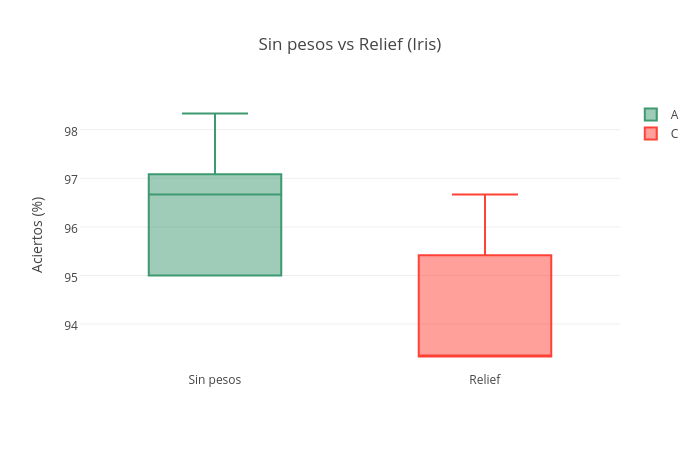
\includegraphics[width=\columnwidth]{no_weights-Relief_Iris}
Figura 1. Conjunto de datos: Iris. Comparación entre 1-NN sin considerar pesos y con la heurística Relief.\\

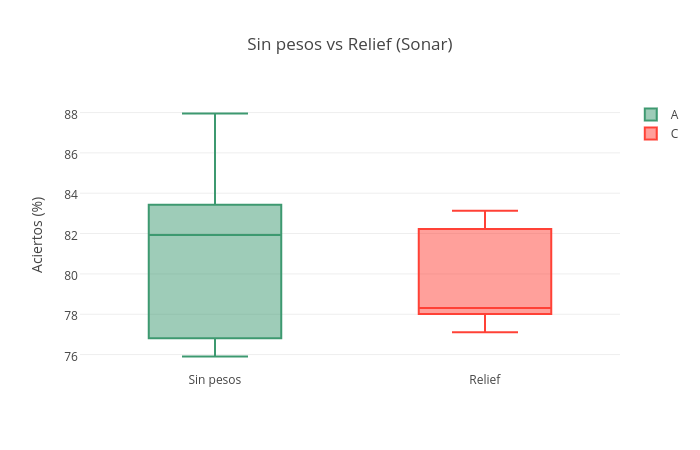
\includegraphics[width=\columnwidth]{no_weights-Relief_Sonar}
Figura 2. Conjunto de datos: Sonar. Comparación entre 1-NN sin considerar pesos y con la heurística Relief.\\

En el caso del conjunto de datos Iris y Sonar (Figura 1 y 2), el porcentaje de aciertos obtenidos al excluir los pesos presentan una mejora poco significativa con respecto a Relief. La diferencia entre ellos es cercano al 2\% en promedio. \\

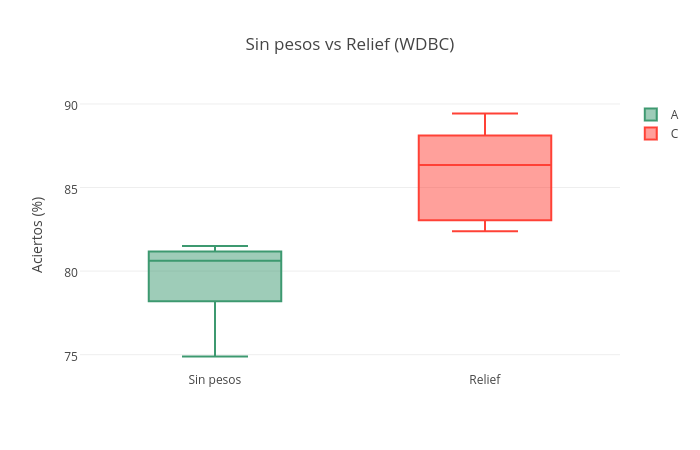
\includegraphics[width=\columnwidth]{no_weights-Relief_WDBC}
Figura 3. Conjunto de datos: WDBC. Comparación entre 1-NN sin considerar pesos y con la heurística Relief.\\

Para Wisconsin Diagnostic Breast Cancer Relief incrementa el promedio del porcentaje de aciertos en apróximadamente 6\% con respecto a "sin pesos"\\

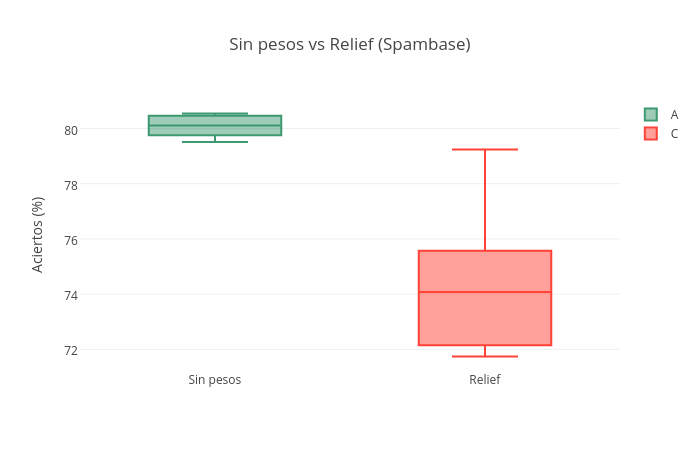
\includegraphics[width=\columnwidth]{no_weights-Relief_Spambase}
Figura 4. Conjunto de datos: Spambase. Comparación entre 1-NN sin considerar pesos y con la heurística Relief.\\

En cuanto a Spambase es evidente que el uso de Relief perjudica la obtención de aciertos, esto se debe probablemente a que contiene datos muy dispersos con varios atributo igual a 0, lo que impide que la heurística diferencie claramente un clase de otra.\\

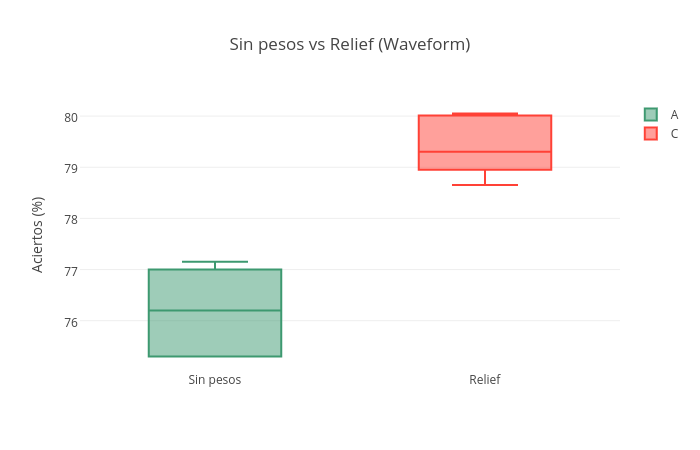
\includegraphics[width=\columnwidth]{no_weights-Relief_Waveform}
Figura 5. Conjunto de datos: Waveform. Comparación entre 1-NN sin considerar pesos y con la heurística Relief.\\

Se puede obeservar que el promedio de aciertos mejora con el uso de Relief en un 4\%. En general, la metaheurística proporciona buenos resultados para los conjuntos de datos utilizados en tiempos aceptables; alrededor de 1 segundo para los conjuntos considerados pequeños (Iris, Sonar y WDBC) y 5 segundos para los grandes (Spambase y Waveform).\\

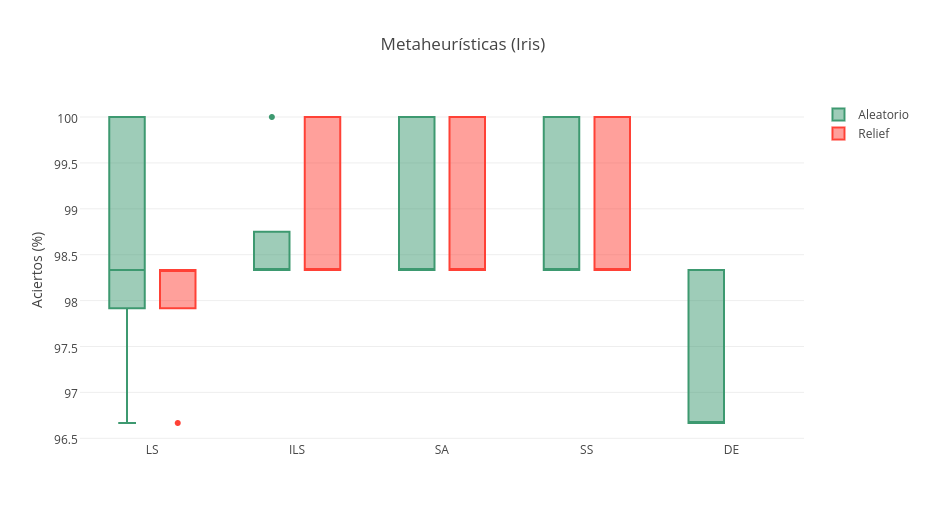
\includegraphics[width=\columnwidth]{metaheuristicas_Iris}
Figura 6. Conjunto de datos: Iris. Comparación entre todas las metaheurísticas.

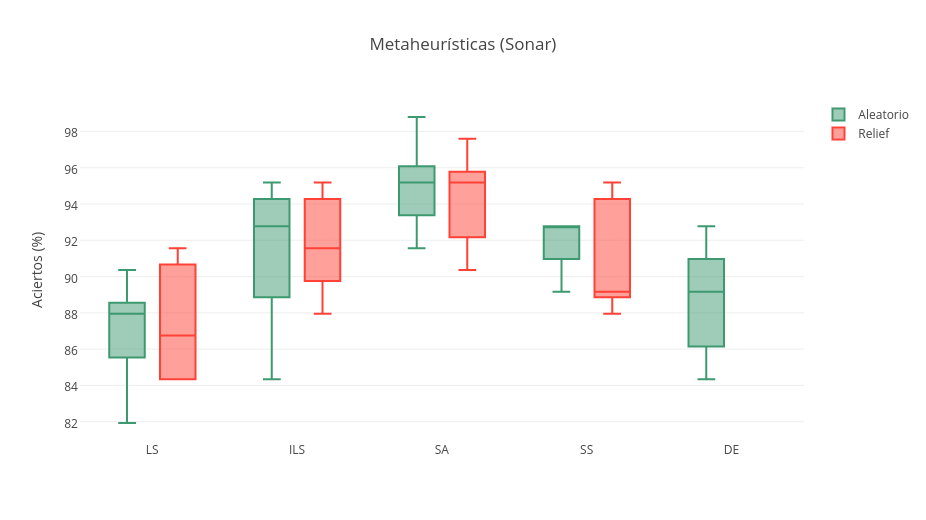
\includegraphics[width=\columnwidth]{metaheuristicas_Sonar}
Figura 7. Conjunto de datos: Sonar. Comparación entre todas las metaheurísticas.

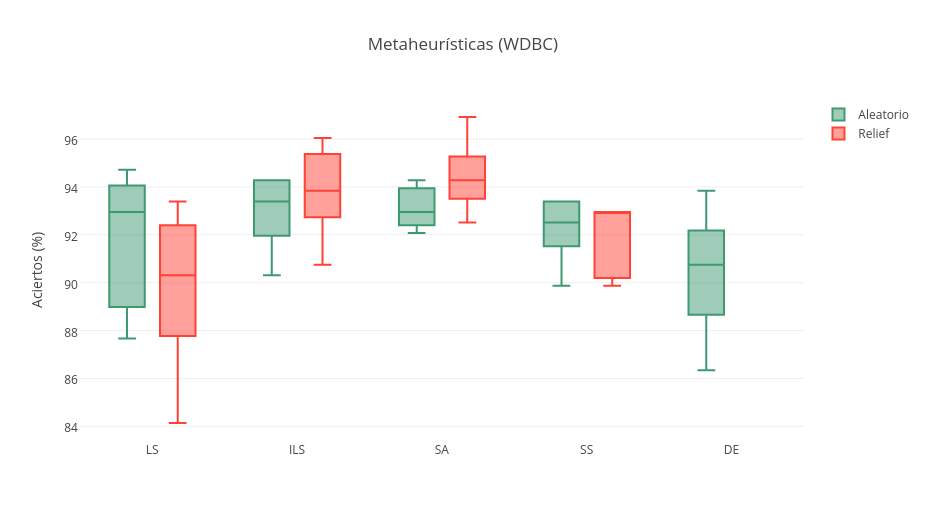
\includegraphics[width=\columnwidth]{metaheuristicas_WDBC}
Figura 8. Conjunto de datos: WDBC. Comparación entre todas las metaheurísticas.

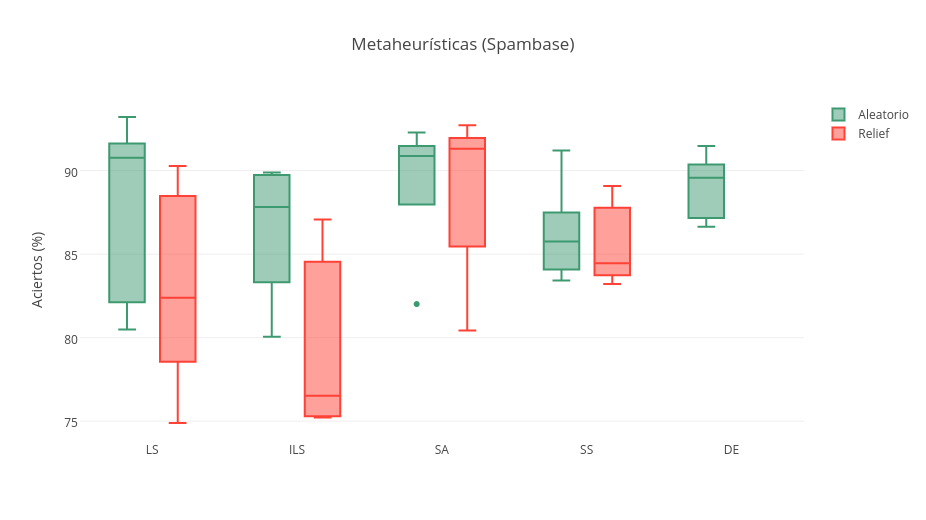
\includegraphics[width=\columnwidth]{metaheuristicas_Spambase}
Figura 9. Conjunto de datos: Spambase. Comparación entre todas las metaheurísticas.

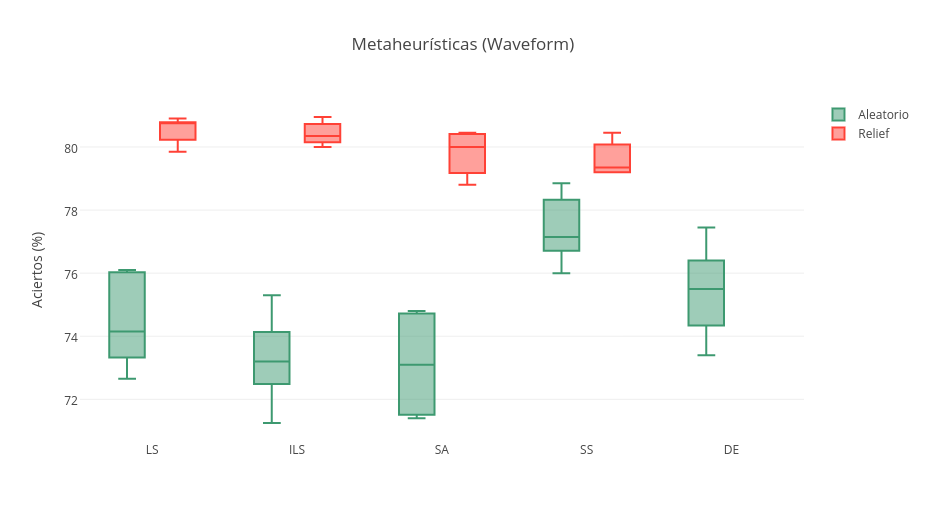
\includegraphics[width=\columnwidth]{metaheuristicas_Waveform}
Figura 10. Conjunto de datos: Waveform. Comparación entre todas las metaheurísticas.

%------------------------------------------------------------------------------%
%                               CONCLUSIONES                                   %
%------------------------------------------------------------------------------%

\section*{Conclusiones}

%perturbar más la solución
%cambiar el alpha del crossover

Aquí concluyen.

%------------------------------------------------------------------------------%
%                               BIBLIOGRAFÍA                                   %
%------------------------------------------------------------------------------%

\small
\bibliographystyle{abbrv}

\begin{thebibliography}{99}

\bibitem{UCI_Waveform}
Breiman, L. (1988). UCI Machine Learning Repository
\newblock [\url{https://archive.ics.uci.edu/ml/machine-learning-databases/waveform/}].
\newblock Irvine, CA: University of California, School of Information and Computer Science.

\bibitem{Cano_2003}
Cano, J. Herrera, F. Lozano. M
\newblock Using evolutionary algorithms as Instance Selection for data
reduction in KDD: an experimental study.
\newblock {\em IEEE Transaction on Evolutionary computation}, 2003.

\bibitem{UCI_Iris}
Fisher, R.A. (1988). UCI Machine Learning Repository
\newblock [\url{https://archive.ics.uci.edu/ml/machine-learning-databases/iris/}].
\newblock Irvine, CA: University of California, School of Information and Computer Science.

\bibitem{Glover_2003}
Glover, F
\newblock Handbook of metaheuristics.
\newblock {\em Operation resarch and management science}, 2003.

\bibitem{Herrera_2017}
Herrera, F.
\newblock Metaheurísticas.
\newblock {\em Seminario 2: Problemas de optimización con técnicas
basadas en búsqueda local}, 2017. Disponible en:
\url{http://sci2s.ugr.es/sites/default/files/files/Teaching/GraduatesCourses/Metaheuristicas/Sem02-Problemas-BusquedaLocal-MHs-16-17.pdf}

\bibitem{UCI_SpamBase}
Hopkins, M. (1999). UCI Machine Learning Repository
\newblock [\url{https://archive.ics.uci.edu/ml/machine-learning-databases/spambase/}].
\newblock Irvine, CA: University of California, School of Information and Computer Science.

\bibitem{Kira_1992}
Kira, K., Rendell, A.
\newblock A practical approach to feature selection, 1992.

\bibitem{Mitchell_1997}
Mitchell, T.
\newblock Machine Learning.
\newblock {\em From Book News, Inc}, 1997.

\bibitem{UCI_Sonar}
Sejnowski, T (año). UCI Machine Learning Repository
\newblock [\url{http://archive.ics.uci.edu/ml/machine-learning-databases/undocumented/connectionist-bench/sonar/}].
\newblock Irvine, CA: University of California, School of Information and Computer Science.

\bibitem{Talbi_2009}
Talbi E.
\newblock Metaheuristics: From desing to implementation
\newblock {\em University of Lille}, 2009.

\bibitem{UCI_WDBC}
Wolberg, W. (1995). UCI Machine Learning Repository
\newblock [\url{https://archive.ics.uci.edu/ml/machine-learning-databases/breast-cancer-wisconsin/}].
\newblock Irvine, CA: University of California, School of Information and Computer Science.

%----TODO: ELIMINAR BIBITEM ----%
%\bibitem{so2005}
%EJEMPLO C. So and H. So.
%\newblock A groundbreaking result.
%\newblock {\em Journal of Everything}, 59(2):23--37, 2005.
%
\end{thebibliography}

%------------------------------------------------------------------------------%
%                                APÉNDICE                                      %
%------------------------------------------------------------------------------%

\newpage
\section*{Apéndice}

\subsection*{Experimento 1}

Tabla 1. Conjunto de Datos: Iris, Algoritmo: LS aleatorio.
Tabla 2. Conjunto de Datos: Iris, Algoritmo: LS relief.
Tabla 3. Conjunto de Datos: Iris, Algoritmo: ILS aleatorio.
Tabla 4. Conjunto de Datos: Iris, Algoritmo: ILS relief.
Tabla 5. Conjunto de Datos: Iris, Algoritmo: SA aleatorio.
Tabla 6. Conjunto de Datos: Iris, Algoritmo: SA relief.
Tabla 7. Conjunto de Datos: Iris, Algoritmo: SS aleatorio.
Tabla 8. Conjunto de Datos: Iris, Algoritmo: SS relief.
Tabla 9. Conjunto de Datos: Iris, Algoritmo: DE.
Tabla 10. Conjunto de Datos: Sonar, Algoritmo: LS aleatorio.
Tabla 11. Conjunto de Datos: Sonar, Algoritmo: LS relief.
Tabla 12. Conjunto de Datos: Sonar, Algoritmo: ILS aleatorio.
Tabla 13. Conjunto de Datos: Sonar, Algoritmo: ILS relief.
Tabla 14. Conjunto de Datos: Sonar, Algoritmo: SA aleatorio.
Tabla 15. Conjunto de Datos: Sonar, Algoritmo: SA relief.
Tabla 16. Conjunto de Datos: Sonar, Algoritmo: SS aleatorio.
Tabla 17. Conjunto de Datos: Sonar, Algoritmo: SS relief.
Tabla 18. Conjunto de Datos: Sonar, Algoritmo: DE.
Tabla 19. Conjunto de Datos: WDBC, Algoritmo: LS aleatorio.
Tabla 20. Conjunto de Datos: WDBC, Algoritmo: LS relief.
Tabla 21. Conjunto de Datos: WDBC, Algoritmo: ILS aleatorio.
Tabla 22. Conjunto de Datos: WDBC, Algoritmo: ILS relief.
Tabla 23. Conjunto de Datos: WDBC, Algoritmo: SA aleatorio.
Tabla 24. Conjunto de Datos: WDBC, Algoritmo: SA relief.
Tabla 25. Conjunto de Datos: WDBC, Algoritmo: SS aleatorio.
Tabla 26. Conjunto de Datos: WDBC, Algoritmo: SS relief.
Tabla 27. Conjunto de Datos: WDBC, Algoritmo: DE.
Tabla 28. Conjunto de Datos: Spambase, Algoritmo: LS aleatorio.
Tabla 29. Conjunto de Datos: Spambase, Algoritmo: LS relief.
Tabla 30. Conjunto de Datos: Spambase, Algoritmo: ILS aleatorio.
Tabla 31. Conjunto de Datos: Spambase, Algoritmo: ILS relief.
Tabla 32. Conjunto de Datos: Spambase, Algoritmo: SA aleatorio.
Tabla 33. Conjunto de Datos: Spambase, Algoritmo: SA relief.
Tabla 34. Conjunto de Datos: Spambase, Algoritmo: SS aleatorio.
Tabla 35. Conjunto de Datos: Spambase, Algoritmo: SS relief.
Tabla 36. Conjunto de Datos: Spambase, Algoritmo: DE.
Tabla 37. Conjunto de Datos: Waveform, Algoritmo: LS aleatorio.
Tabla 38. Conjunto de Datos: Waveform, Algoritmo: LS relief.
Tabla 39. Conjunto de Datos: Waveform, Algoritmo: ILS aleatorio.
Tabla 40. Conjunto de Datos: Waveform, Algoritmo: ILS relief.
Tabla 41. Conjunto de Datos: Waveform, Algoritmo: SA aleatorio.
Tabla 42. Conjunto de Datos: Waveform, Algoritmo: SA relief.
Tabla 43. Conjunto de Datos: Waveform, Algoritmo: SS aleatorio.
Tabla 44. Conjunto de Datos: Waveform, Algoritmo: SS relief.
Tabla 45. Conjunto de Datos: Waveform, Algoritmo: DE.

\subsection*{Experimento 2}

Tabla 46. Conjunto de Datos: Iris, Algoritmo: Sin pesos.
Tabla 47. Conjunto de Datos: Iris, Algoritmo: Relief.
Tabla 48. Conjunto de Datos: Iris, Algoritmo: LS aleatorio.
Tabla 49. Conjunto de Datos: Iris, Algoritmo: LS relief.
Tabla 50. Conjunto de Datos: Iris, Algoritmo: ILS aleatorio.
Tabla 51. Conjunto de Datos: Iris, Algoritmo: ILS relief.
Tabla 52. Conjunto de Datos: Iris, Algoritmo: SA aleatorio.
Tabla 53. Conjunto de Datos: Iris, Algoritmo: SA relief.
Tabla 54. Conjunto de Datos: Iris, Algoritmo: SS aleatorio.
Tabla 55. Conjunto de Datos: Iris, Algoritmo: SS relief.
Tabla 56. Conjunto de Datos: Iris, Algoritmo: DE.
Tabla 57. Conjunto de Datos: Sonar, Algoritmo: Sin pesos.
Tabla 58. Conjunto de Datos: Sonar, Algoritmo: Relief.
Tabla 59. Conjunto de Datos: Sonar, Algoritmo: LS aleatorio.
Tabla 60. Conjunto de Datos: Sonar, Algoritmo: LS relief.
Tabla 61. Conjunto de Datos: Sonar, Algoritmo: ILS aleatorio.
Tabla 62. Conjunto de Datos: Sonar, Algoritmo: ILS relief.
Tabla 63. Conjunto de Datos: Sonar, Algoritmo: SA aleatorio.
Tabla 64. Conjunto de Datos: Sonar, Algoritmo: SA relief.
Tabla 65. Conjunto de Datos: Sonar, Algoritmo: SS aleatorio.
Tabla 66. Conjunto de Datos: Sonar, Algoritmo: SS relief.
Tabla 67. Conjunto de Datos: Sonar, Algoritmo: DE.
Tabla 68. Conjunto de Datos: WDBC, Algoritmo: Sin pesos.
Tabla 69. Conjunto de Datos: WDBC, Algoritmo: Relief.
Tabla 70. Conjunto de Datos: WDBC, Algoritmo: LS aleatorio.
Tabla 71. Conjunto de Datos: WDBC, Algoritmo: LS relief.
Tabla 72. Conjunto de Datos: WDBC, Algoritmo: ILS aleatorio.
Tabla 73. Conjunto de Datos: WDBC, Algoritmo: ILS relief.
Tabla 74. Conjunto de Datos: WDBC, Algoritmo: SA aleatorio.
Tabla 75. Conjunto de Datos: WDBC, Algoritmo: SA relief.
Tabla 76. Conjunto de Datos: WDBC, Algoritmo: SS aleatorio.
Tabla 77. Conjunto de Datos: WDBC, Algoritmo: SS relief.
Tabla 78. Conjunto de Datos: WDBC, Algoritmo: DE.
Tabla 79. Conjunto de Datos: Spambase, Algoritmo: Sin pesos.
Tabla 80. Conjunto de Datos: Spambase, Algoritmo: Relief.
Tabla 81. Conjunto de Datos: Spambase, Algoritmo: LS aleatorio.
Tabla 82. Conjunto de Datos: Spambase, Algoritmo: LS relief.
Tabla 83. Conjunto de Datos: Spambase, Algoritmo: ILS aleatorio.
Tabla 84. Conjunto de Datos: Spambase, Algoritmo: ILS relief.
Tabla 85. Conjunto de Datos: Spambase, Algoritmo: SA aleatorio.
Tabla 86. Conjunto de Datos: Spambase, Algoritmo: SA relief.
Tabla 87. Conjunto de Datos: Spambase, Algoritmo: SS aleatorio.
Tabla 88. Conjunto de Datos: Spambase, Algoritmo: SS relief.
Tabla 89. Conjunto de Datos: Spambase, Algoritmo: DE.
Tabla 90. Conjunto de Datos: Waveform, Algoritmo: Sin pesos.
Tabla 91. Conjunto de Datos: Waveform, Algoritmo: Relief.
Tabla 92. Conjunto de Datos: Waveform, Algoritmo: LS aleatorio.
Tabla 93. Conjunto de Datos: Waveform, Algoritmo: LS relief.
Tabla 94. Conjunto de Datos: Waveform, Algoritmo: ILS aleatorio.
Tabla 95. Conjunto de Datos: Waveform, Algoritmo: ILS relief.
Tabla 96. Conjunto de Datos: Waveform, Algoritmo: SA aleatorio.
Tabla 97. Conjunto de Datos: Waveform, Algoritmo: SA relief.
Tabla 98. Conjunto de Datos: Waveform, Algoritmo: SS aleatorio.
Tabla 99. Conjunto de Datos: Waveform, Algoritmo: SS relief.
Tabla 100. Conjunto de Datos: Waveform, Algoritmo: DE.


%\csvreader[
%  respect all,
%  autotabular
%  ]{statistics/iris/no_weights.csv}{}{\csvlinetotablerow}%
%\\
%\csvreader[
%  respect all,
%  autotabular
%  ]{statistics/sonar/no_weights.csv}{}{\csvlinetotablerow}%
%\\
%\csvreader[
%  respect all,
%  autotabular
%  ]{statistics/spambase/no_weights.csv}{}{\csvlinetotablerow}%
%\\
%\csvreader[
%  respect all,
%  autotabular
%  ]{statistics/wdbc/no_weights.csv}{}{\csvlinetotablerow}%
%\\
%RELIEF\\
%\csvreader[
%  respect all,
%  autotabular
%  ]{statistics/iris/relief.csv}{}{\csvlinetotablerow}%
%\\
%\csvreader[
%  respect all,
%  autotabular
%  ]{statistics/sonar/relief.csv}{}{\csvlinetotablerow}%
%\\
%\csvreader[
%  respect all,
%  autotabular
%  ]{statistics/spambase/relief.csv}{}{\csvlinetotablerow}%
%\\
%\csvreader[
%  respect all,
%  autotabular
%  ]{statistics/wdbc/relief.csv}{}{\csvlinetotablerow}%


%------------------------ EL EJEMPLO DE LA PROFE -----------------------------%
%
%\section{La sección de ejemplo de la profe}
%Citan así~\cite{so2005}. ELIMINAR AL ESCRIBIR EL INFORME
%
%\begin{algorithm}
% \DontPrintSemicolon
% \vspace*{0.1cm}
% \KwIn{Descripcion}
% \KwOut{Descripcion}
% Primer paso\;
% Segundo\;
% \ForEach{$i = 1\dots n$}{
%  \If{Alguna condición}{
%   Algo aqui\;
%   }
% }
% \KwRet{Valor}
% \vspace*{0.1cm}
% \caption{Nombre}
%\end{algorithm}
%
\end{document}
